\documentclass{standalone}
\usepackage{tikz}
\usetikzlibrary{patterns, positioning}


\begin{document}
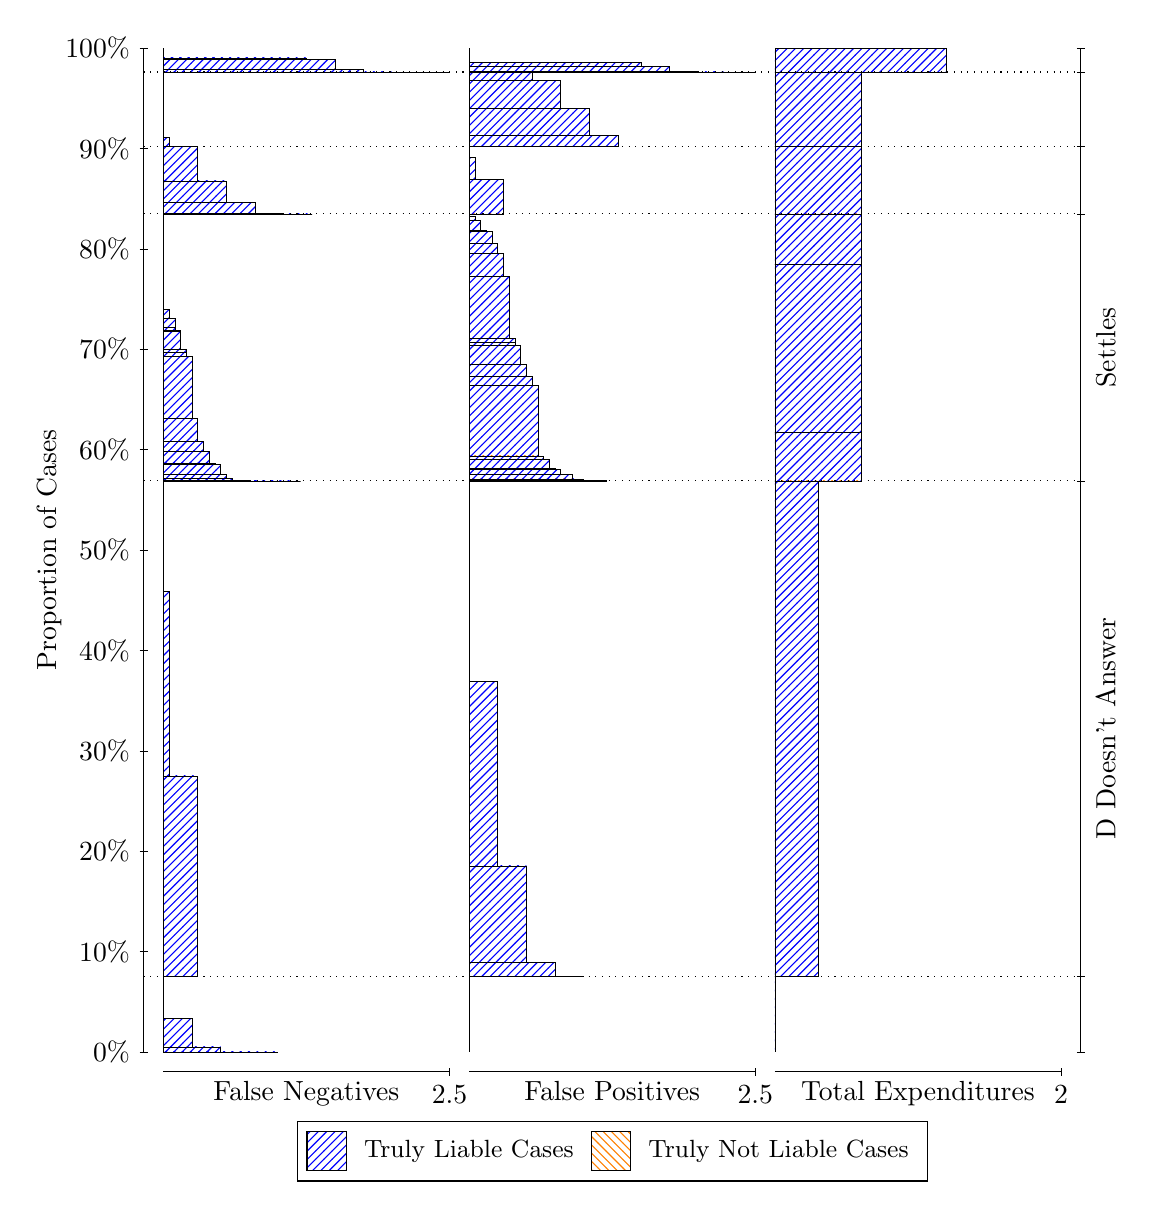
\begin{tikzpicture}
\draw[black, very thin] (1.5,1.75) -- (1.5,14.5);
\node[rotate=90, text=black, anchor=center] at (0.3, 8.125) {Proportion of Cases};
\draw[black, very thin] (1.45,1.75) -- (1.55,1.75);
\node[text=black, anchor=east] at (1.45, 1.75) {0\%};
\draw[black, very thin] (1.45,3.025) -- (1.55,3.025);
\node[text=black, anchor=east] at (1.45, 3.025) {10\%};
\draw[black, very thin] (1.45,4.3) -- (1.55,4.3);
\node[text=black, anchor=east] at (1.45, 4.3) {20\%};
\draw[black, very thin] (1.45,5.575) -- (1.55,5.575);
\node[text=black, anchor=east] at (1.45, 5.575) {30\%};
\draw[black, very thin] (1.45,6.85) -- (1.55,6.85);
\node[text=black, anchor=east] at (1.45, 6.85) {40\%};
\draw[black, very thin] (1.45,8.125) -- (1.55,8.125);
\node[text=black, anchor=east] at (1.45, 8.125) {50\%};
\draw[black, very thin] (1.45,9.4) -- (1.55,9.4);
\node[text=black, anchor=east] at (1.45, 9.4) {60\%};
\draw[black, very thin] (1.45,10.675) -- (1.55,10.675);
\node[text=black, anchor=east] at (1.45, 10.675) {70\%};
\draw[black, very thin] (1.45,11.95) -- (1.55,11.95);
\node[text=black, anchor=east] at (1.45, 11.95) {80\%};
\draw[black, very thin] (1.45,13.225) -- (1.55,13.225);
\node[text=black, anchor=east] at (1.45, 13.225) {90\%};
\draw[black, very thin] (1.45,14.5) -- (1.55,14.5);
\node[text=black, anchor=east] at (1.45, 14.5) {100\%};

\draw[black, very thin] (13.4,1.75) -- (13.4,14.5);
\draw[black, very thin] (13.35,1.75) -- (13.45,1.75);
\node[anchor=west] at (13.35, 1.75) {};
\draw[black, very thin] (13.35,2.709) -- (13.45,2.709);
\node[anchor=west] at (13.35, 2.709) {};
\draw[black, very thin] (13.35,9.0026) -- (13.45,9.0026);
\node[anchor=west] at (13.35, 9.0026) {};
\draw[black, very thin] (13.35,12.395) -- (13.45,12.395);
\node[anchor=west] at (13.35, 12.395) {};
\draw[black, very thin] (13.35,13.253) -- (13.45,13.253);
\node[anchor=west] at (13.35, 13.253) {};
\draw[black, very thin] (13.35,14.195) -- (13.45,14.195);
\node[anchor=west] at (13.35, 14.195) {};
\draw[black, very thin] (13.35,14.5) -- (13.45,14.5);
\node[anchor=west] at (13.35, 14.5) {};

\draw[black, very thin, pattern color=blue, pattern=north east lines] (1.75,1.75) rectangle (3.2033,1.75);
\draw[black, very thin, pattern color=blue, pattern=north east lines] (1.75,1.75) rectangle (2.84,1.7505);
\draw[black, very thin, pattern color=blue, pattern=north east lines] (1.75,1.7505) rectangle (2.4767,1.8142);
\draw[black, very thin, pattern color=blue, pattern=north east lines] (1.75,1.8142) rectangle (2.1133,2.1765);
\draw[black, very thin, pattern color=orange, pattern=north west lines] (1.75,2.1765) rectangle (1.75,2.1765);
\draw[black, very thin, pattern color=blue, pattern=north east lines] (1.75,2.1765) rectangle (1.75,2.709);
\draw[black, very thin, pattern color=blue, pattern=north east lines] (1.75,2.709) rectangle (2.186,5.2569);
\draw[black, very thin, pattern color=blue, pattern=north east lines] (1.75,5.2569) rectangle (1.8227,7.5989);
\draw[black, very thin, pattern color=orange, pattern=north west lines] (1.75,7.5989) rectangle (1.75,7.5989);
\draw[black, very thin, pattern color=blue, pattern=north east lines] (1.75,7.5989) rectangle (1.75,9.0026);
\draw[black, very thin, pattern color=blue, pattern=north east lines] (1.75,9.0026) rectangle (3.494,9.0026);
\draw[black, very thin, pattern color=blue, pattern=north east lines] (1.75,9.0026) rectangle (3.3487,9.0026);
\draw[black, very thin, pattern color=blue, pattern=north east lines] (1.75,9.0026) rectangle (3.2033,9.0026);
\draw[black, very thin, pattern color=blue, pattern=north east lines] (1.75,9.0026) rectangle (3.1307,9.0028);
\draw[black, very thin, pattern color=blue, pattern=north east lines] (1.75,9.0028) rectangle (3.058,9.0028);
\draw[black, very thin, pattern color=blue, pattern=north east lines] (1.75,9.0028) rectangle (3.058,9.0028);
\draw[black, very thin, pattern color=blue, pattern=north east lines] (1.75,9.0028) rectangle (2.9853,9.003);
\draw[black, very thin, pattern color=blue, pattern=north east lines] (1.75,9.003) rectangle (2.9127,9.0031);
\draw[black, very thin, pattern color=blue, pattern=north east lines] (1.75,9.0031) rectangle (2.84,9.0053);
\draw[black, very thin, pattern color=blue, pattern=north east lines] (1.75,9.0053) rectangle (2.7673,9.0105);
\draw[black, very thin, pattern color=blue, pattern=north east lines] (1.75,9.0105) rectangle (2.6947,9.0107);
\draw[black, very thin, pattern color=blue, pattern=north east lines] (1.75,9.0107) rectangle (2.6947,9.0151);
\draw[black, very thin, pattern color=blue, pattern=north east lines] (1.75,9.0151) rectangle (2.622,9.0151);
\draw[black, very thin, pattern color=blue, pattern=north east lines] (1.75,9.0151) rectangle (2.622,9.0387);
\draw[black, very thin, pattern color=blue, pattern=north east lines] (1.75,9.0387) rectangle (2.5493,9.0837);
\draw[black, very thin, pattern color=blue, pattern=north east lines] (1.75,9.0837) rectangle (2.4767,9.2099);
\draw[black, very thin, pattern color=blue, pattern=north east lines] (1.75,9.2099) rectangle (2.404,9.2161);
\draw[black, very thin, pattern color=blue, pattern=north east lines] (1.75,9.2161) rectangle (2.404,9.2264);
\draw[black, very thin, pattern color=blue, pattern=north east lines] (1.75,9.2264) rectangle (2.3313,9.231);
\draw[black, very thin, pattern color=blue, pattern=north east lines] (1.75,9.231) rectangle (2.3313,9.3747);
\draw[black, very thin, pattern color=blue, pattern=north east lines] (1.75,9.3747) rectangle (2.3313,9.3748);
\draw[black, very thin, pattern color=blue, pattern=north east lines] (1.75,9.3748) rectangle (2.2587,9.3848);
\draw[black, very thin, pattern color=blue, pattern=north east lines] (1.75,9.3848) rectangle (2.2587,9.5028);
\draw[black, very thin, pattern color=blue, pattern=north east lines] (1.75,9.5028) rectangle (2.186,9.7938);
\draw[black, very thin, pattern color=blue, pattern=north east lines] (1.75,9.7938) rectangle (2.1133,10.586);
\draw[black, very thin, pattern color=blue, pattern=north east lines] (1.75,10.586) rectangle (2.0407,10.636);
\draw[black, very thin, pattern color=blue, pattern=north east lines] (1.75,10.636) rectangle (2.0407,10.673);
\draw[black, very thin, pattern color=blue, pattern=north east lines] (1.75,10.673) rectangle (1.968,10.676);
\draw[black, very thin, pattern color=blue, pattern=north east lines] (1.75,10.676) rectangle (1.968,10.905);
\draw[black, very thin, pattern color=blue, pattern=north east lines] (1.75,10.905) rectangle (1.968,10.911);
\draw[black, very thin, pattern color=blue, pattern=north east lines] (1.75,10.911) rectangle (1.8953,10.956);
\draw[black, very thin, pattern color=blue, pattern=north east lines] (1.75,10.956) rectangle (1.8953,11.069);
\draw[black, very thin, pattern color=blue, pattern=north east lines] (1.75,11.069) rectangle (1.8227,11.177);
\draw[black, very thin, pattern color=orange, pattern=north west lines] (1.75,11.177) rectangle (1.75,11.177);
\draw[black, very thin, pattern color=blue, pattern=north east lines] (1.75,11.177) rectangle (1.75,12.395);
\draw[black, very thin, pattern color=blue, pattern=north east lines] (1.75,12.395) rectangle (3.6393,12.395);
\draw[black, very thin, pattern color=blue, pattern=north east lines] (1.75,12.395) rectangle (3.276,12.398);
\draw[black, very thin, pattern color=blue, pattern=north east lines] (1.75,12.398) rectangle (2.9127,12.54);
\draw[black, very thin, pattern color=blue, pattern=north east lines] (1.75,12.54) rectangle (2.5493,12.812);
\draw[black, very thin, pattern color=blue, pattern=north east lines] (1.75,12.812) rectangle (2.186,13.253);
\draw[black, very thin, pattern color=orange, pattern=north west lines] (1.75,13.253) rectangle (1.75,13.253);
\draw[black, very thin, pattern color=blue, pattern=north east lines] (1.75,13.253) rectangle (2.186,13.255);
\draw[black, very thin, pattern color=blue, pattern=north east lines] (1.75,13.255) rectangle (1.8227,13.362);
\draw[black, very thin, pattern color=orange, pattern=north west lines] (1.75,13.362) rectangle (1.75,13.362);
\draw[black, very thin, pattern color=blue, pattern=north east lines] (1.75,13.362) rectangle (1.75,14.195);
\draw[black, very thin, pattern color=blue, pattern=north east lines] (1.75,14.195) rectangle (5.3833,14.195);
\draw[black, very thin, pattern color=blue, pattern=north east lines] (1.75,14.195) rectangle (5.02,14.195);
\draw[black, very thin, pattern color=blue, pattern=north east lines] (1.75,14.195) rectangle (4.6567,14.197);
\draw[black, very thin, pattern color=blue, pattern=north east lines] (1.75,14.197) rectangle (4.2933,14.228);
\draw[black, very thin, pattern color=blue, pattern=north east lines] (1.75,14.228) rectangle (3.93,14.352);
\draw[black, very thin, pattern color=blue, pattern=north east lines] (1.75,14.352) rectangle (3.5667,14.374);
\draw[black, very thin, pattern color=blue, pattern=north east lines] (1.75,14.374) rectangle (3.2033,14.374);
\draw[black, very thin, pattern color=blue, pattern=north east lines] (1.75,14.374) rectangle (2.404,14.374);
\draw[black, very thin, pattern color=blue, pattern=north east lines] (1.75,14.374) rectangle (2.0407,14.374);
\draw[black, very thin, pattern color=orange, pattern=north west lines] (1.75,14.374) rectangle (1.75,14.374);
\draw[black, very thin, pattern color=blue, pattern=north east lines] (1.75,14.374) rectangle (1.75,14.5);
\draw[black, very thin, pattern color=orange, pattern=north west lines] (5.6333,1.75) rectangle (5.6333,1.75);
\draw[black, very thin, pattern color=blue, pattern=north east lines] (5.6333,1.75) rectangle (5.6333,2.709);
\draw[black, very thin, pattern color=orange, pattern=north west lines] (5.6333,2.709) rectangle (7.0867,2.709);
\draw[black, very thin, pattern color=blue, pattern=north east lines] (5.6333,2.709) rectangle (7.0867,2.7106);
\draw[black, very thin, pattern color=blue, pattern=north east lines] (5.6333,2.7106) rectangle (6.7233,2.8831);
\draw[black, very thin, pattern color=blue, pattern=north east lines] (5.6333,2.8831) rectangle (6.36,4.1127);
\draw[black, very thin, pattern color=blue, pattern=north east lines] (5.6333,4.1127) rectangle (5.9967,6.4547);
\draw[black, very thin, pattern color=blue, pattern=north east lines] (5.6333,6.4547) rectangle (5.6333,9.0026);
\draw[black, very thin, pattern color=orange, pattern=north west lines] (5.6333,9.0026) rectangle (7.3773,9.0026);
\draw[black, very thin, pattern color=blue, pattern=north east lines] (5.6333,9.0026) rectangle (7.3773,9.0083);
\draw[black, very thin, pattern color=orange, pattern=north west lines] (5.6333,9.0083) rectangle (7.232,9.0083);
\draw[black, very thin, pattern color=blue, pattern=north east lines] (5.6333,9.0083) rectangle (7.232,9.0137);
\draw[black, very thin, pattern color=orange, pattern=north west lines] (5.6333,9.0137) rectangle (7.0867,9.0137);
\draw[black, very thin, pattern color=blue, pattern=north east lines] (5.6333,9.0137) rectangle (7.0867,9.0248);
\draw[black, very thin, pattern color=blue, pattern=north east lines] (5.6333,9.0248) rectangle (7.014,9.0287);
\draw[black, very thin, pattern color=orange, pattern=north west lines] (5.6333,9.0287) rectangle (6.9413,9.0287);
\draw[black, very thin, pattern color=blue, pattern=north east lines] (5.6333,9.0287) rectangle (6.9413,9.0834);
\draw[black, very thin, pattern color=blue, pattern=north east lines] (5.6333,9.0834) rectangle (6.8687,9.0873);
\draw[black, very thin, pattern color=orange, pattern=north west lines] (5.6333,9.0873) rectangle (6.796,9.0873);
\draw[black, very thin, pattern color=blue, pattern=north east lines] (5.6333,9.0873) rectangle (6.796,9.1527);
\draw[black, very thin, pattern color=blue, pattern=north east lines] (5.6333,9.1527) rectangle (6.7233,9.165);
\draw[black, very thin, pattern color=orange, pattern=north west lines] (5.6333,9.165) rectangle (6.6507,9.165);
\draw[black, very thin, pattern color=blue, pattern=north east lines] (5.6333,9.165) rectangle (6.6507,9.277);
\draw[black, very thin, pattern color=blue, pattern=north east lines] (5.6333,9.277) rectangle (6.578,9.3091);
\draw[black, very thin, pattern color=blue, pattern=north east lines] (5.6333,9.3091) rectangle (6.5053,9.3208);
\draw[black, very thin, pattern color=orange, pattern=north west lines] (5.6333,9.3208) rectangle (6.5053,9.3208);
\draw[black, very thin, pattern color=blue, pattern=north east lines] (5.6333,9.3208) rectangle (6.5053,10.22);
\draw[black, very thin, pattern color=blue, pattern=north east lines] (5.6333,10.22) rectangle (6.4327,10.328);
\draw[black, very thin, pattern color=orange, pattern=north west lines] (5.6333,10.328) rectangle (6.36,10.328);
\draw[black, very thin, pattern color=blue, pattern=north east lines] (5.6333,10.328) rectangle (6.36,10.486);
\draw[black, very thin, pattern color=blue, pattern=north east lines] (5.6333,10.486) rectangle (6.2873,10.725);
\draw[black, very thin, pattern color=orange, pattern=north west lines] (5.6333,10.725) rectangle (6.2147,10.725);
\draw[black, very thin, pattern color=blue, pattern=north east lines] (5.6333,10.725) rectangle (6.2147,10.761);
\draw[black, very thin, pattern color=blue, pattern=north east lines] (5.6333,10.761) rectangle (6.2147,10.811);
\draw[black, very thin, pattern color=blue, pattern=north east lines] (5.6333,10.811) rectangle (6.142,10.815);
\draw[black, very thin, pattern color=blue, pattern=north east lines] (5.6333,10.815) rectangle (6.142,11.603);
\draw[black, very thin, pattern color=blue, pattern=north east lines] (5.6333,11.603) rectangle (6.0693,11.894);
\draw[black, very thin, pattern color=blue, pattern=north east lines] (5.6333,11.894) rectangle (5.9967,12.022);
\draw[black, very thin, pattern color=blue, pattern=north east lines] (5.6333,12.022) rectangle (5.924,12.171);
\draw[black, very thin, pattern color=blue, pattern=north east lines] (5.6333,12.171) rectangle (5.8513,12.181);
\draw[black, very thin, pattern color=blue, pattern=north east lines] (5.6333,12.181) rectangle (5.8513,12.187);
\draw[black, very thin, pattern color=blue, pattern=north east lines] (5.6333,12.187) rectangle (5.7787,12.187);
\draw[black, very thin, pattern color=blue, pattern=north east lines] (5.6333,12.187) rectangle (5.7787,12.313);
\draw[black, very thin, pattern color=blue, pattern=north east lines] (5.6333,12.313) rectangle (5.706,12.358);
\draw[black, very thin, pattern color=blue, pattern=north east lines] (5.6333,12.358) rectangle (5.6333,12.395);
\draw[black, very thin, pattern color=orange, pattern=north west lines] (5.6333,12.395) rectangle (6.0693,12.395);
\draw[black, very thin, pattern color=blue, pattern=north east lines] (5.6333,12.395) rectangle (6.0693,12.836);
\draw[black, very thin, pattern color=blue, pattern=north east lines] (5.6333,12.836) rectangle (5.706,13.108);
\draw[black, very thin, pattern color=blue, pattern=north east lines] (5.6333,13.108) rectangle (5.6333,13.253);
\draw[black, very thin, pattern color=orange, pattern=north west lines] (5.6333,13.253) rectangle (7.5227,13.253);
\draw[black, very thin, pattern color=blue, pattern=north east lines] (5.6333,13.253) rectangle (7.5227,13.391);
\draw[black, very thin, pattern color=blue, pattern=north east lines] (5.6333,13.391) rectangle (7.1593,13.73);
\draw[black, very thin, pattern color=blue, pattern=north east lines] (5.6333,13.73) rectangle (6.796,14.087);
\draw[black, very thin, pattern color=blue, pattern=north east lines] (5.6333,14.087) rectangle (6.4327,14.194);
\draw[black, very thin, pattern color=blue, pattern=north east lines] (5.6333,14.194) rectangle (6.0693,14.195);
\draw[black, very thin, pattern color=orange, pattern=north west lines] (5.6333,14.195) rectangle (9.2667,14.195);
\draw[black, very thin, pattern color=blue, pattern=north east lines] (5.6333,14.195) rectangle (9.2667,14.195);
\draw[black, very thin, pattern color=orange, pattern=north west lines] (5.6333,14.195) rectangle (8.9033,14.195);
\draw[black, very thin, pattern color=blue, pattern=north east lines] (5.6333,14.195) rectangle (8.9033,14.196);
\draw[black, very thin, pattern color=orange, pattern=north west lines] (5.6333,14.196) rectangle (8.54,14.196);
\draw[black, very thin, pattern color=blue, pattern=north east lines] (5.6333,14.196) rectangle (8.54,14.203);
\draw[black, very thin, pattern color=orange, pattern=north west lines] (5.6333,14.203) rectangle (8.1767,14.203);
\draw[black, very thin, pattern color=blue, pattern=north east lines] (5.6333,14.203) rectangle (8.1767,14.263);
\draw[black, very thin, pattern color=blue, pattern=north east lines] (5.6333,14.263) rectangle (7.8133,14.315);
\draw[black, very thin, pattern color=blue, pattern=north east lines] (5.6333,14.315) rectangle (7.45,14.322);
\draw[black, very thin, pattern color=blue, pattern=north east lines] (5.6333,14.322) rectangle (7.0867,14.322);
\draw[black, very thin, pattern color=blue, pattern=north east lines] (5.6333,14.322) rectangle (6.7233,14.322);
\draw[black, very thin, pattern color=orange, pattern=north west lines] (5.6333,14.322) rectangle (5.924,14.322);
\draw[black, very thin, pattern color=blue, pattern=north east lines] (5.6333,14.322) rectangle (5.924,14.322);
\draw[black, very thin, pattern color=orange, pattern=north west lines] (5.6333,14.322) rectangle (5.6333,14.322);
\draw[black, very thin, pattern color=blue, pattern=north east lines] (5.6333,14.322) rectangle (5.6333,14.5);
\draw[black, very thin, pattern color=orange, pattern=north west lines] (9.5167,1.75) rectangle (9.5167,1.75);
\draw[black, very thin, pattern color=blue, pattern=north east lines] (9.5167,1.75) rectangle (9.5167,2.709);
\draw[black, very thin, pattern color=orange, pattern=north west lines] (9.5167,2.709) rectangle (10.062,2.709);
\draw[black, very thin, pattern color=blue, pattern=north east lines] (9.5167,2.709) rectangle (10.062,9.0026);
\draw[black, very thin, pattern color=orange, pattern=north west lines] (9.5167,9.0026) rectangle (10.607,9.0026);
\draw[black, very thin, pattern color=blue, pattern=north east lines] (9.5167,9.0026) rectangle (10.607,9.6155);
\draw[black, very thin, pattern color=orange, pattern=north west lines] (9.5167,9.6155) rectangle (10.607,9.6155);
\draw[black, very thin, pattern color=blue, pattern=north east lines] (9.5167,9.6155) rectangle (10.607,11.753);
\draw[black, very thin, pattern color=orange, pattern=north west lines] (9.5167,11.753) rectangle (10.607,11.753);
\draw[black, very thin, pattern color=blue, pattern=north east lines] (9.5167,11.753) rectangle (10.607,12.395);
\draw[black, very thin, pattern color=orange, pattern=north west lines] (9.5167,12.395) rectangle (10.607,12.395);
\draw[black, very thin, pattern color=blue, pattern=north east lines] (9.5167,12.395) rectangle (10.607,13.253);
\draw[black, very thin, pattern color=orange, pattern=north west lines] (9.5167,13.253) rectangle (10.607,13.253);
\draw[black, very thin, pattern color=blue, pattern=north east lines] (9.5167,13.253) rectangle (10.607,14.195);
\draw[black, very thin, pattern color=orange, pattern=north west lines] (9.5167,14.195) rectangle (11.697,14.195);
\draw[black, very thin, pattern color=blue, pattern=north east lines] (9.5167,14.195) rectangle (11.697,14.5);
\draw[black, dotted] (1.5,2.709) -- (13.4,2.709);
\draw[black, dotted] (1.5,9.0026) -- (13.4,9.0026);
\draw[black, dotted] (1.5,12.395) -- (13.4,12.395);
\draw[black, dotted] (1.5,13.253) -- (13.4,13.253);
\draw[black, dotted] (1.5,14.195) -- (13.4,14.195);
\draw[black, very thin] (1.75,1.5) -- (5.3833,1.5);
\node[text=black, anchor=north] at (3.5667, 1.5) {False Negatives};
\draw[black, very thin] (5.3833,1.45) -- (5.3833,1.55);
\node[text=black, anchor=north] at (5.3833, 1.45) {2.5};

\draw[black, very thin] (5.6333,1.5) -- (9.2667,1.5);
\node[text=black, anchor=north] at (7.45, 1.5) {False Positives};
\draw[black, very thin] (9.2667,1.45) -- (9.2667,1.55);
\node[text=black, anchor=north] at (9.2667, 1.45) {2.5};

\draw[black, very thin] (9.5167,1.5) -- (13.15,1.5);
\node[text=black, anchor=north] at (11.333, 1.5) {Total Expenditures};
\draw[black, very thin] (13.15,1.45) -- (13.15,1.55);
\node[text=black, anchor=north] at (13.15, 1.45) {2};


\node[text=black, centered, rotate=90] at (13.72, 5.8558) {D Doesn't Answer};
\node[text=black, centered, rotate=90] at (13.72, 10.699) {Settles};




\draw (7.449999999999999,1.5) node[draw=none] (baseCoordinate) {};
\begin{scope}[align=center]
        \matrix[scale=0.5, draw=black, below=0.5cm of baseCoordinate, nodes={draw}, column sep=0.1cm]{
            \node[rectangle, draw, minimum width=0.5cm, minimum height=0.5cm, pattern color=blue, pattern=north east lines] {}; &
            \node[draw=none, font=\small, text=black] (B) {Truly Liable Cases}; &
            \node[rectangle, draw, minimum width=0.5cm, minimum height=0.5cm, pattern color=orange, pattern=north west lines] {}; &
            \node[draw=none, font=\small, text=black] (B) {Truly Not Liable Cases}; \\
            };
\end{scope}

\end{tikzpicture}
\end{document}